\documentclass[12pt, a4paper]{report}
\usepackage[top=3cm, bottom=3cm, left=4cm,right=3cm]{geometry}
\usepackage{setspace} %interlineado
\setlength{\parindent}{7mm} % sangria
\setlength{\parskip}{\baselineskip} %espacio entre parrafos
\usepackage{microtype} %realiza micro-arreglos en los parrafos para que queden mejor justificados
%\renewcommand{\rmdefault}{phv} % Arial
%\renewcommand{\sfdefault}{phv} % Arial
\usepackage{placeins} % ayuda a que las tablas no queden en medio de los textos
\usepackage{tabulary} %tabla que ajusta celdas al texto
\usepackage[font={footnotesize}]{caption} % tamano para la descripcion de las tablas
\captionsetup{labelformat=empty} % elimina el prefijo de los nombres de las tablas
\usepackage{array}
\usepackage{float}
\usepackage{makecell}
\usepackage{graphicx}
\usepackage[spanish,es-tabla]{babel}
\usepackage[authoryear,datebegin]{flexbib}
\bibliographystyle{flexbib}
\usepackage{fancyhdr}%header de los capitulos
\fancyhead{}
\fancyhead[L]{\nouppercase{\leftmark}}

\newcommand{\membrete}{
	
\includegraphics[width=0.15\textwidth]{./img/logo-uc.png}~\\[1cm]

	UNIVERSIDAD DE CARABOBO \\	
	Facultad Experimental de Ciencias y Tecnolog\'{i}a\\
	Departamento de Computaci\'{o}n
	\vfill
	\textbf{SOFTWARE PARA EL ESPECTROFOT\'{O}METRO MINISCAN XE PLUS USADO EN EL DIAGN\'{O}STICO DE PATOLOG\'{I}AS DERMATOL\'{O}GICAS EN PACIENTES. CASO DE ESTUDIO: CIMBUC.}
}

\newcommand{\autor}{
	\textbf{Autor:}\\
	Gabriel A. N\'{u}\~{n}ez N.\\
}

\newcommand{\tutores}{
	\textbf{Tutores:} \\
	Prof. Patricia Guerrero \\
	Prof. Harold Vasquez
}
%\newcommand{\titulo}{\textbf{SOFTWARE PARA EL ESPECTROFOT\'{O}METRO MINISCAN XE PLUS USADO EN EL DIAGN\'{O}STICO DE PATOLOG\'{I}%AS DERMATOL\'{O}GICAS EN PACIENTES. CASO DE ESTUDIO: CIMBUC.}}

\newcommand{\fecha}{Naguanagua, \today.}

\newcommand{\anchotabla}{14cm}

\newcommand{\altocelda}{2pt}

%\newcommand{\sangriareferencias}{\hspace{7mm}}

%\newcommand{\espacioreferencias}{\vspace{2.5mm}}

\renewcommand\thechapter{\Roman{chapter}}

\renewcommand\thesection{\arabic{chapter}.\arabic{section}}

\selectlanguage{spanish}

\begin{document}
	\begin{titlepage}
	\begin{center}
	\membrete
	\vfill
	\textbf{Autor:}\\
	Gabriel A. N\'{u}\~{n}ez N.\\
	\vfill
	\textbf{Tutores:} \\
	Prof. Patricia Guerrero \\
	Prof. Harold Vasquez
	\vfill
	\fecha
	\end{center}
\end{titlepage}
	\begin{titlepage}
	\begin{center}
	\membrete
	\vfill
	Trabajo Especial de Grado\\
	\titulo
	\vfill
	\textbf{Autor:}\\
	Gabriel A. N\'{u}\~{n}ez N.\\
	\vfill
	\textbf{Tutores:} \\
	Prof. Patricia Guerrero \\
	Prof. Harold Vasquez
	\vfill
	Trabajo Especial de Grado presentado ante la ilustre Universidad de Carabobo, como credencial para optar por el t\'{i}tulo de Licenciado en Computaci\'{o}n.
	\vfill
	\fecha
	\end{center}
\end{titlepage}
	\chapter*{Dedicatoria}

A mi abuela, quien me cri\'{o} desde mis cuatro meses de vida, y a quien llamo mam\'{a} desde que tengo uso de la raz\'{o}n. Este trabajo es para ti, representa la culminaci\'{o}n de una etapa donde estuviste presente d\'{i}a a d\'{i}a, gracias por el \'{a}nimo, los consejos y los valores que me has inculcado, por haberme ense\~{n}ado que con Dios de la mano todo se puede, por haber salido adelante conmigo, por haberme hecho el hombre de bien que soy hoy, por todos los sacrificios que hiciste en silencio, y m\'{a}s que nada por todo el amor que has brindado. Te amo mam\'{a}.

\begin{flushright}
	\textbf{Gabriel A. N\'{u}\~{n}ez N.}
\end{flushright}

	\chapter*{Agradecimientos}

	A Dios, por acompa\~{n}arme en todo momento, por ser mi mejor maestro, y por haberme ayudado a alcanzar esta meta, la culminaci\'{o}n de mi carrera.

	A mi familia, por apoyarme en todo momento, por estar presente para celebrar los logros, compartir la alegr\'{i}a y superar las dificultades.

	A mis amigos, quienes me ayudaron a tomar las cosas con calma, me ayudaron a despejar mi mente innumerables veces, y me dieron el \'{a}nimo necesario para terminar este largo trayecto a tiempo.

	A mi profesora Patricia, por haberme ayudado y aconsejado desde el primero hasta el \'{u}ltimo d\'{i}a de este recorrido, y haberme mostrado que siempre se pueden mejorar las cosas.

	A mi profesor Harold, por saber cu\'{a}ndo exigirme m\'{a}s, ser justo, y mostrarme el nivel de excelencia que puedo alcanzar, a pesar de la distancia.

	Al equipo de profesores e investigadores que hace vida en el CIMBUC, por haberme brindado una experiencia \'{u}nica al trabajar con ellos.

	A la empresa HunterLab, por haber respondido todas mis dudas, y por haberme proporcionado la ayuda que necesit\'{e} e incluso m\'{a}s.


\begin{flushright}
	\textbf{Gabriel A. N\'{u}\~{n}ez N.}
\end{flushright}

	\renewenvironment{abstract}{
  \vspace*{\fill}
  \begin{center}%
    \bfseries\abstractname
  \end{center}}%

\begin{abstract}
	\noindent
El espectrofot\'{o}metro de reflexi\'{o}n difusa, denominado MiniScan XE Plus, es un instrumento de medici\'{o}n utilizado por el Centro de Investigaciones M\'{e}dicas y Biotecnol\'{o}gicas de la Universidad de Carabobo (CIMBUC), que ayuda a los dermat\'{o}logos a establecer diagn\'{o}sticos sobre patolog\'{i}as en la piel de pacientes, de manera precisa y sin necesidad de realizar biopsias. No obstante, el software comercial disponible para la utilizaci\'{o}n de tal instrumento es poco amigable, dif\'{i}cil de utilizar e imposible de modificar y extender. La presente investigaci\'{o}n tiene como objetivo desarrollar un software amigable, modificable y extensible, que se ajuste a las necesidades de los dermat\'{o}logos y que garantice un mejor aprovechamiento del instrumento en cuesti\'{o}n.

	\noindent
	\textbf{Palabras claves:} espectrofot\'{o}metro, an\'{a}lisis bioqu\'{i}mico de la piel, biopsia, software privativo, software libre.
	\vfill
\end{abstract}

\vfill

\selectlanguage{english}
\begin{abstract}
	\noindent
The diffuse reflectance spectrophotometer, called MiniScan XE Plus, is a measurement instrument used by the Medical Research and Biotechnology Center at the University of Carabobo (CIMBUC), which helps dermatologists to establish pathologies diagnoses in the skin of patients precisely, without need for biopsy. However, the available commercial software for the use of such an instrument is unfriendly, difficult to use and impossible to modify and extend. This research aims to develop a friendly, modifiable and expandable software that meets the needs of dermatologists and ensures a better use of the instrument itself.

	\noindent
	\textbf{Keywords:} spectrophotometer, biochemical analysis of the skin, biopsy, privative software, open source software.
	\vfill
\end{abstract}

\selectlanguage{spanish}
	\pagestyle{fancy}
	\chapter*{Introducci\'{o}n}

\addcontentsline{toc}{chapter}{Introducci\'{o}n}

	La espectroscop\'{i}a de reflectancia difusa es una t\'{e}cnica \'{o}ptica con la cual es  posible estudiar las propiedades bioqu\'{i}micas y las condiciones estructurales de un tejido biol\'{o}gico. Los instrumentos que emplean t\'{e}cnicas como \'{e}sta son de gran ayuda para los dermat\'{o}logos, raz\'{o}n por la cual tales instrumentos han tomado suma importancia en el \'{a}rea de la medicina dermatol\'{o}gica.

El Centro de Investigaciones M\'{e}dicas y Biotecnol\'{o}gicas de la Universidad de Carabobo (CIMBUC) dispone de un espectrofot\'{o}metro de reflexi\'{o}n difusa denominado MiniScan XE Plus. Este instrumento se utiliza a trav\'{e}s del \'{u}nico software disponible para su manejo, designado HunterLab Universal Software.

El HunterLab Universal Software es un software comercial y privativo que fue descontinuado en el a\~{n}o 2008. Su interfaz gr\'{a}fica de usuario est\'{a} en ingl\'{e}s y contiene m\'{a}s funciones de las necesarias para manejar el instrumento en estudio, lo que lo hace poco amigable y dif\'{i}cil de entender por los dermat\'{o}logos.

Esta investigaci\'{o}n se centr\'{o} en desarrollar un software amigable, modificable y extensible para la utilizaci\'{o}n del MiniScan XE Plus, ajustandose a las necesidades de los dermat\'{o}logos, a fin de sentar una base que permite la realizaci\'{o}n de nuevas investigaciones que conlleven a la implementaci\'{o}n de t\'{e}cnicas que empleen an\'{a}lisis m\'{a}s complejos, y como resultado, diagn\'{o}sticos m\'{a}s completos y diversos sobre patolog\'{i}as dermatol\'{o}gicas presentes en pacientes.

\newpage
\thispagestyle{plain}
	El presente trabajo de investigaci\'{o}n est\'{a} estructurado en cinco cap\'{i}tulos, los cuales son descritos a continuaci\'{o}n.

	El \textbf{cap\'{i}tulo I} describe el contexto de la problem\'{a}tica que motiva el desarrollo de este trabajo de investigaci\'{o}n, se indican los objetivos a cumplir con el mismo y se explican las razones que justifican la necesidad de su realizaci\'{o}n.

	En el \textbf{cap\'{i}tulo II} se presentan los trabajos que anteceden esta investigaci\'{o}n, las observaciones directas realizadas para llevarla a cabo, y se explican las bases te\'{o}ricas que sustentan el desarrollo de las funciones que debe ofrecer el software producto de la misma.

	En el \textbf{cap\'{i}tulo III} se describen la metodolog\'{i}a de investigaci\'{o}n y la metodolog\'{i}a de desarrollo que se emplearon para planificar, dise\~{n}ar y desarrollar el software propuesto en el presente trabajo de investigaci\'{o}n.

	El \textbf{cap\'{i}tulo IV} muestra los resultados que fueron alcanzados en el desarrollo del presente trabajo de investigaci\'{o}n, incluyendo las fases metodol\'{o}gicas, las tecnolog\'{i}as y los recursos utilizados, la interfaz gr\'{a}fica de usuario del software resultante y las pruebas realizadas.

	Finalmente, en el \textbf{cap\'{i}tulo V} se establecen las conclusiones a las que se lleg\'{o} con el presente trabajo de investigaci\'{o}n, y las recomendaciones consideradas a tomar para trabajos futuros, tomando en cuenta dichas conclusiones.

	
	
	\newpage
	\spacing{1.5} % interlineado
	\chapter{\label{cap:1}El Problema}

	\section{Planteamiento del Problema}	
\cite{Bersha} indica que durante el diagn\'{o}stico de enfermedades de la piel, la observaci\'{o}n cuidadosa y la evaluaci\'{o}n visual del \'{a}rea sospechada es siempre el primer paso y el m\'{a}s importante. Esto es seguido generalmente por una escisi\'{o}n o biopsia por punci\'{o}n, en la que se extrae una muestra de tejido de la piel para un an\'{a}lisis microsc\'{o}pico. La observaci\'{o}n visual suele ser subjetiva y los pacientes a menudo se someten a cicatrices y dolor durante la escisi\'{o}n. Por otro lado, las t\'{e}cnicas \'{o}pticas son por lo general no invasivas y los resultados de estas son a menudo objetivos. Durante el diagn\'{o}stico no invasivo no se crea ninguna ruptura en la piel, y los pacientes no se someten al dolor y a cicatrices durante el tratamiento.

Los avances tecnol\'{o}gicos en la actualidad permiten emplear t\'{e}cnicas de \'{o}ptica con la capacidad de estudiar  las propiedades estructurales y bioqu\'{i}micas del tejido biol\'{o}gico de manera precisa y no invasiva. Los instrumentos que emplean tales t\'{e}cnicas son de gran ayuda para los m\'{e}dicos dermat\'{o}logos, raz\'{o}n por la cual han tomado suma importancia en el \'{a}rea m\'{e}dica dermatol\'{o}gica.

Hoy d\'{i}a existen diferentes tipos de estudios \'{o}pticos in-situ, in-vivo e invitro del tejido biol\'{o}gico, como lo es la espectroscop\'{i}a de reflectancia difusa. Con esta t\'{e}cnica es  posible estudiar las propiedades bioqu\'{i}micas y las condiciones estructurales de un tejido biol\'{o}gico, analizando la interacci\'{o}n luz-tejido de una manera no invasiva \cite{Perez-Gallardo}.

En este sentido, el Centro de Investigaciones M\'{e}dicas y Biotecnol\'{o}gicas de la Universidad de Carabobo (CIMBUC) dispone de un Espectrofot\'{o}metro de reflexi\'{o}n difusa denominado ``MiniScan XE Plus''. La empresa ``HunterLab'', creadora y distribuidora del ``MiniScan XE Plus'', lo describe como un instrumento utilizado para medir la transmisi\'{o}n y/o reflectancia de espec\'{i}menes, como una funci\'{o}n de longitud de onda, que aplica una t\'{e}cnica llamada espectroscop\'{i}a de reflectancia difusa. 

Ahora bien, para emplear el uso del instrumento en estudio, el CIMBUC ha tenido que utilizar el software comercial disponible para la utilizaci\'{o}n del mismo, denominado ``HunterLab Universal Software'', el cual es un software propietario de 16-bit dise\~{n}ado para el Sistema Operativo Microsoft Windows Version 3.x, con la posibilidad de ejecutarse en Windows 95, Windows 2000 y Windows NT, y el mismo fue descontinuado en el a\~{n}o 2008. Este software ofrece un conjunto de funcionalidades que abarcan no s\'{o}lo la utilizaci\'{o}n del Espectrofot\'{o}metro, sino tambi\'{e}n la utilizaci\'{o}n de otros instrumentos ofrecidos por la empresa ``HunterLab''. La interfaz gr\'{a}fica de usuario de dicho software esta en idioma ingl\'{e}s. Por \'{u}ltimo, los resultados que genera este software no poseen el formato de gesti\'{o}n de informaci\'{o}n de pacientes con el que trabajan los dermat\'{o}logos del CIMBUC.

Tomando en cuenta lo mencionado anteriormente se tiene que el software comercial es propietario y est\'{a} descontinuado, por lo tanto no existe la posibilidad de modificarlo, mejorarlo ni extenderlo; ofrece funcionalidades ajenas al uso exclusivo del Espectrofot\'{o}metro, causando que la interfaz gr\'{a}fica de usuario contenga m\'{a}s opciones disponibles de las necesarias para manejar el instrumento en estudio. Asimismo, como consecuencia de que la interfaz gr\'{a}fica de usuario est\'{e} en idioma ingl\'{e}s, \'{e}sta es dif\'{i}cil de entender por los dermat\'{o}logos. Aunado al hecho de que los resultados generados por dicho software no poseen el formato con el que trabajan los dermat\'{o}logos, haciendo necesario su traspaso manual, lo que produce a una ralentizaci\'{o}n en las consultas con pacientes. Todo esto conlleva a que los m\'{e}dicos requieran de asistencia t\'{e}cnica entrenada, disponible en todo momento para guiar el uso apropiado del software.

De lo antedicho se desprende que, el software comercial en utilizaci\'{o}n para el manejo del Espectrofot\'{o}metro posee una interfaz gr\'{a}fica de usuario poco amigable, y el costo del tiempo de capacitaci\'{o}n para su uso correcto podr\'{i}a ser alto. \'{E}ste software no podr\'{a} modificarse, mejorarse ni extenderse por el hecho de ser propietario, y por lo tanto no se fomentar\'{a} el uso del instrumento en cuesti\'{o}n en el campo m\'{e}dico (p\'{u}blico o privado). De igual manera, tampoco se fomentar\'{a} el desarrollo de nuevas aplicaciones que utilicen sus resultados como insumo, sosegando as\'{i} la posibilidad de realizar an\'{a}lisis m\'{a}s complejos y de proveer a los dermat\'{o}logos de resultados que les permitan establecer diagn\'{o}sticos m\'{a}s completos.

Motivado a todo lo anterior, se desarroll\'{o} un nuevo software para el Espectrofot\'{o}metro, con una interfaz gr\'{a}fica de usuario amigable, utilizando los lineamientos de la ingenier\'{i}a del software pertinentes y favoreciendo su integraci\'{o}n con nuevas aplicaciones que se desarrollen en proyectos futuros, logrando as\'{i} el nivel deseado de amigabilidad y extensibilidad.

Con esta investigaci\'{o}n se espera fomentar la utilizaci\'{o}n del nuevo software, una mejor capacitaci\'{o}n del personal m\'{e}dico para su debido uso y el aporte de una base s\'{o}lida sobre la cual se podr\'{a}n desarrollar nuevos proyectos.

	\section{Justificaci\'{o}n}
El estudio y diagn\'{o}stico de patolog\'{i}as dermatol\'{o}gicas en pacientes es un \'{a}rea cuyo campo est\'{a} en constante desarrollo, requiriendo que los procesos involucrados en \'{e}sta no solamente sean de calidad, sino que sean capaces de desarrollarse a la par; el software utilizado en dicha \'{a}rea no es una excepci\'{o}n. Que los dermat\'{o}logos experimenten dificultades al momento de utilizar el ``HunterLab Universal Software'' debido a que el mismo este en ingl\'{e}s, ofrezca funciones ajenas al instrumento en estudio, no emplee el formato de historia m\'{e}dica utilizado por ellos, y que adem\'{a}s no ofrezca la posibilidad de modificarlo, mejorarlo ni agregarle nuevas funciones, es un problema grave, ya que no s\'{o}lo ralentiza cada consulta con un paciente, sino que genera la necesidad de asistencia t\'{e}cnica disponible en todo momento para la debida utilizaci\'{o}n de dicho software; por \'{u}ltimo y no menos importante, disminuye el nivel de aprovechamiento potencial del instrumento de medici\'{o}n en estudio.

Con respecto a software de calidad, \cite{Sommerville} explica lo siguiente: As\'{i} como los servicios que proveen, los productos de software tienen cierto n\'{u}mero de atributos asociados que reflejan la calidad de ese software. Estos atributos no est\'{a}n directamente relacionados con lo que el software hace. M\'{a}s bien, reflejan su comportamiento durante su ejecuci\'{o}n, en la estructura y organizaci\'{o}n del programa fuente, y en la documentaci\'{o}n asociada. Ejemplos de estos atributos son el tiempo de respuesta del software a una pregunta del usuario y la comprensi\'{o}n del programa fuente.

El conjunto espec\'{i}fico de atributos que se espera de un software depende obviamente de su aplicaci\'{o}n. Esto se generaliza en el conjunto de atributos que se muestran en la Tabla 1, la cual contiene las caracter\'{i}sticas esenciales de un software bien dise\~{n}ado.

	\begin{table}[htb]
		\small
		\centering
		\setlength{\extrarowheight}{5pt}
		\begin{tabulary}{15cm}{|c|L|}
			\hline
			\textbf{Caracter\'{i}stica} & \textbf{Descripci\'{o}n}\\ \hline
			\textbf{Mantenibilidad} & El software debe describirse de tal forma que pueda evolucionar  para cumplir las necesidades de cambio de los 					clientes. Este es un atributo cr\'{i}tico, debido a que el cambio en el software es una consecuencia inevitable de un cambio en el entorno de negocios.\\ \hline
			\textbf{Confiabilidad} & La confiabilidad del software tiene un gran n\'{u}mero de caracter\'{i}sticas, incluyendo la fiabilidad, protecci\'{o}n y seguridad. El software confiable no debe causar da\~{n}os f\'{i}sicos o econ\'{o}micos en el caso de una falla del sistema.\\ \hline
			\textbf{Eficiencia} & El software no debe hacer que se malgasten los recursos del sistema, como la memoria y los ciclos de procesamiento. Por lo tanto, la eficiencia incluye tiempos de respuesta y de procesamiento, utilizaci\'{o}n de la memoria, etc\'{e}tera.\\ \hline
			\textbf{Usabilidad} & El software debe ser f\'{a}cil de utilizar, sin esfuerzo adicional por el usuario para quien est\'{a} dise\~{n}ado. Esto significa que debe tener una interfaz gr\'{a}fica de usuario apropiada y una documentaci\'{o}n adecuada.\\ \hline
		\end{tabulary}
			\caption{\textbf{Tabla 1.} \textit{Atributos esenciales de un buen software}		(Fuente: Sommerville, 2005).}
	\end{table}
			\FloatBarrier %you shall not pass table!!
Debido a que el ``HunterLab Universal Software'' es propietario, el CIMBUC no dispone del c\'{o}digo fuente del mismo, lo que se traduce en la inexistencia del primer atributo esencial para un buen software: la mantenibilidad; ya que el software propietario no puede ser cambiado ni adaptarse a necesidades espec\'{i}ficas. Por la misma raz\'{o}n de ser un software propietario del cual no se tiene el c\'{o}digo fuente, no se puede determinar con certidumbre el segundo atributo: la confiabilidad; debido a que no se puede evaluar completamente el nivel de protecci\'{o}n y seguridad existentes en dicho software. Por \'{u}ltimo y no menos importante, la usabilidad del software existente es baja, ya que la interfaz gr\'{a}fica de usuario es poco amigable, haciendo surgir la necesidad de disponer de personal t\'{e}cnico para la utilizaci\'{o}n correcta del mismo. Por estas razones, se desarroll\'{o} un software que cumpliese con los atributos esenciales que debe poseer un buen software.

\cite{Sommerville} se\~{n}ala que un dise\~{n}o cuidadoso de la interfaz gr\'{a}fica de usuario es parte fundamental del proceso de dise\~{n}o general del software. Si un software debe alcanzar su potencial m\'{a}ximo, es fundamental que su interfaz gr\'{a}fica de usuario sea dise\~{n}ada para ajustarse a las habilidades, experiencia y expectativas de sus usuarios previstos. Un buen dise\~{n}o de la interfaz gr\'{a}fica de usuario es cr\'{i}tico para la confiabilidad del software. Muchos de los llamados ``errores de usuario'' son causados por el hecho de que las interfaces gr\'{a}ficas de usuario no consideran las habilidades de los usuarios reales y su entorno de trabajo.

El dise\~{n}o de la interfaz gr\'{a}fica de usuario del ``HunterLab Universal Software'' es la principal raz\'{o}n por la cual los dermat\'{o}logos requieren de personal t\'{e}cnico que los asista al momento de utilizarlo. Esto porque dicha interfaz est\'{a} en idioma ingl\'{e}s, contiene funcionalidades que no son necesarias para la utilizaci\'{o}n de Espectrofot\'{o}metro y no proporciona el formato con el que trabajan los dermat\'{o}logos, lo que dificulta la utilizaci\'{o}n de dicha interfaz. Por estas razones los dermat\'{o}logos perciben este software comercial como no intuitivo, ni auto descriptivo ni amigable, temiendo cometer errores al utilizarlo por su propia cuenta y generar resultados err\'{o}neos, poniendo en riesgo el diagn\'{o}stico, y en consecuencia, la salud de los pacientes en consulta.

En conclusi\'{o}n, siguiendo los lineamientos de dise\~{n}o y calidad del software que se consideraron pertinentes, se desarroll\'{o} un software amigable, modificable y extensible, el cual ofrece las funciones que necesitan los dermat\'{o}logos para establecer diagn\'{o}sticos, emplea el formato de historia m\'{e}dica con el que trabajan, permite la exportaci\'{o}n de los resultados a un formato de archivo portable; por \'{u}ltimo y no menos importante, se cre\'{o} una base sobre la cual se prodr\'{a}n trabajar proyectos futuros que necesiten utilizar los resultados de este software como insumo.
	\newpage

	\section{Objetivos de la Investigaci\'{o}n}
En la siguiente secci\'{o}n se especifican los objetivos del trabajo, distinguiendo entre el objetivo general y los objetivos espec\'{i}ficos.
		\subsection{Objetivo General}
	Desarrollar un software para el Espectrofot\'{o}metro ``MiniScan XE Plus'', usado en el diagn\'{o}stico de patolog\'{i}as dermatol\'{o}gicas en pacientes, tomando como caso de estudio el CIMBUC.
		\subsection{Objetivos Espec\'{i}ficos}
			\begin{itemize}
				\item Investigar el estado del arte referente a las caracter\'{i}sticas de software para Espectrofot\'{o}metros de reflexi\'{o}n difusa, dise\~{n}o y calidad de software.
				\item Seleccionar una metodolog\'{i}a que gu\'{i}e el dise\~{n}o y desarrollo del nuevo software para el Espectrofot\'{o}metro ``MiniScan XE Plus''.
				\item Dise\~{n}ar el nuevo software siguiendo la metodolog\'{i}a seleccionada.
				\item Desarrollar el nuevo software, siguiendo la metodolog\'{i}a seleccionada.
				\item Dise\~{n}ar las pruebas para el nuevo software.
				\item Elaborar el manual de usuario del nuevo software.
			\end{itemize}
	\newpage
	\chapter{\label{cap:2}Marco Te\'{o}rico}

	\section{Antecedentes}	
		\begin{itemize}
			\item Por agregar.
		\end{itemize}

	\section{Observaci\'{o}n Directa}
		\begin{itemize}
			\item \textbf{HunterLab Universal Software:} Es un software propietario de 16-bit dise\~{n}ado para el Sistema Operativo Microsoft Windows Version 3.x, con la posibilidad de ejecutarse en Windows 95, Windows 2000, Windows NT y Windows XP, descontinuado en el a\~{n}o 2008. Este software dispone de algunas de funcionalidades desarrolladas en el nuevo software, raz\'{o}n por la cual es una importante referencia.
		
			\item \textbf{MiniScanXE Plus OCX Kit:} Es un archivo de control ActiveX dise\~{n}ado por HunterLab para controlar y/o realizar mediciones con el ``MiniScan XE Plus'', utilizando Visual Basic for Applications (VBA). Su principal objetivo es proveer a los desarrolladores con un componente reutilizable de software que da acceso a las caracteristicas m\'{a}s comunmente utilizadas por el instrumento. La interfaz p\'{u}blica que expone este archivo es utilizada para realizar la comunicaci\'{o}n entre el ``MiniScan XE Plus'' y el nuevo software.
		\end{itemize}
	\newpage
	\chapter{\label{cap:3}Marco Metodol\'{o}gico}

	\section{Metodolog\'{i}a Investigaci\'{o}n-Acci\'{o}n}
	\cite{Baskerville} define la Investigaci\'{o}n-Acci\'{o}n como un m\'{e}todo de investigaci\'{o}n que a finales de la d\'{e}cada de los 90 empez\'{o} a crecer en popularidad, para el uso en investigaciones acad\'{e}micas de sistemas de informaci\'{o}n. Este m\'{e}todo produce resultados de investigaci\'{o}n altamente relevantes, debido a que se fundamenta en la acci\'{o}n pr\'{a}ctica, dirigida a resolver un problema mientras se informa cuidadosamente sobre la teor\'{i}a.

	Esta metodolog\'{i}a tiene una doble finalidad: generar un beneficio al cliente de la investigaci\'{o}n y al mismo tiempo, generar conocimiento de investigaci\'{o}n relevante. Por lo tanto, es una forma de investigar de car\'{a}cter colaborativo que busca unir teor\'{i}a y la pr\'{a}ctica entre investigadores y practicantes, mediante un proceso de naturaleza c\'{i}clica.

	La representaci\'{o}n m\'{a}s habitual de la Investigaci\'{o}n-Acci\'{o}n es la descrita por \cite{Baskerville}, en forma de cinco fases que conforman un ciclo, las cuales se describen en la Figura 1.

\FloatBarrier %you shall not pass table!!
\vline
	\begin{figure}
		\centering
		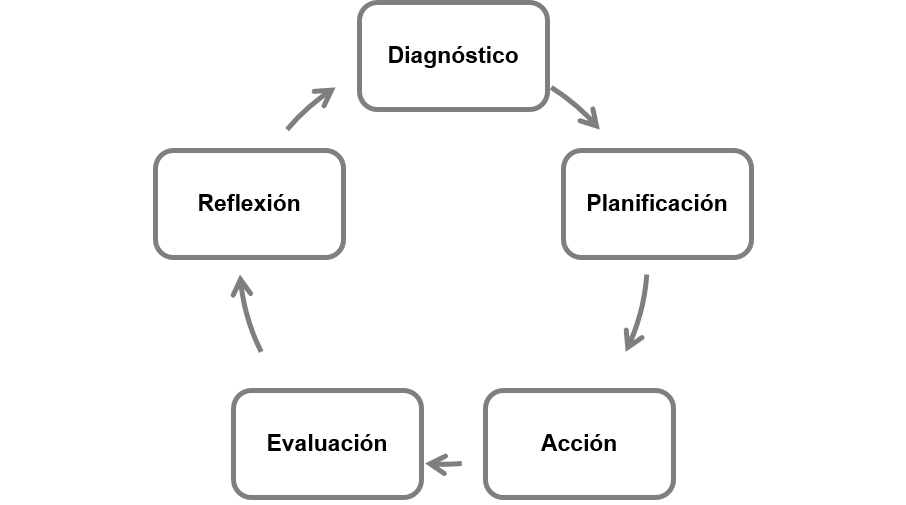
\includegraphics[scale=0.77]{img/investigacion-accion.png}
			\caption{\textbf{Figura 1.} \textit{Car\'{a}cter c\'{i}clico de Investigaci\'{o}n-Acci\'{o}n} (Fuente: Baskerville, 1999).}
	\end{figure}
\FloatBarrier %you shall not pass table!!

	\begin{itemize}
		\item \textbf{Fase de diagn\'{o}stico:} se realiza el proceso de identificaci\'{o}n de los problemas primarios de la investigaci\'{o}n.
		\item \textbf{Fase de planificaci\'{o}n:} se especifican las acciones que se llevaran a cabo para solucionar los problemas primarios.
		\item \textbf{Fase de acci\'{o}n:} se ejecutan las acciones planificadas en la fase anterior.
		\item \textbf{Fase de evaluaci\'{o}n u observaci\'{o}n:} se efect\'{u}a una evaluaci\'{o}n de los resultados obtenidos, para observar, conocer y documentar los efectos de las acciones que fueron realizadas.
		\item \textbf{Fase de reflexi\'{o}n:} se toman los conocimientos adquiridos en la investigaci\'{o}n-acci\'{o}n. Si las acciones ejecutadas no fueron exitosas, los conocimientos pueden proporcionar la base para el diagn\'{o}stico de un nuevo ciclo de investigaci\'{o}n-acci\'{o}n.
	\end{itemize}

En la Tabla 2 se muestran las actividades de la presente investigaci\'{o}n, haciendo correspondencia a cada una de las fases de la Investigaci\'{o}n-Acci\'{o}n descritas por \cite{Baskerville}.

\FloatBarrier %you shall not pass table!!
\vline
	\begin{table}[htb]
		\small
		\centering
		\setlength{\extrarowheight}{5pt}
		\begin{tabulary}{15cm}{|c|L|}
			\hline
			\thead{\textbf{\small{Fase}}} & \thead{\textbf{\small{Actividades}}}\\ \hline
			\textbf{Diagn\'{o}stico} & Identificar los problemas y limitaciones que presenta el HunterLab Universal Software.\\ \hline
			\textbf{Planificaci\'{o}n} & Seleccionar la metodolog\'{i}a de desarrollo, determinar los requisitos del software y realizar un plan de trabajo.
\\ \hline
			\textbf{Acci\'{o}n} & Desarrollar el software, tomando en cuenta los requisitos identificados previamente, los lineamientos de dise\~{n}o y de calidad del software.\\ \hline
			\textbf{Evaluaci\'{o}n} & Realizar las pruebas de funcionalidad e interfaz gr\'{a}fica de usuario del nuevo software.\\ \hline
			\textbf{Reflexi\'{o}n} & Presentar los resultados y los an\'{a}lisis de las pruebas realizadas.\\ \hline
		\end{tabulary}
		\caption{\textbf{Tabla 2.} \textit{Actividades del proyecto seg\'{u}n metodolog\'{i}a Investigaci\'{o}n-Acci\'{o}n} (Fuente: Elaboraci\'{o}n propia).}
	\end{table}
\FloatBarrier %you shall not pass table!!

	\section{Metodolog\'{i}a de Desarrollo de Software}
Para que el desarrollo del nuevo software cumpliera con los objetivos propuestos la presente investigaci\'{o}n, y tomando en cuenta los lineamientos planteados por la ingenier\'{i}a del software, se realiz\'{o} una revisi\'{o}n del enfoque que deber\'{i}a tener la metodolog\'{i}a de desarrollo a utilizar.

Seg\'{u}n \cite{Sommerville}, en los a\~{n}os 80 y a principios de los 90, exist\'{i}a una opini\'{o}n general de que la mejor forma de obtener un mejor software era a trav\'{e}s de una planificaci\'{o}n cuidadosa del proyecto, una garant\'{i}a de calidad formalizada, la utilizaci\'{o}n de m\'{e}todos de an\'{a}lisis y dise\~{n}o soportados por herramientas \textit{CASE}, y por medio de procesos de desarrollo de software controlados y rigurosos. El software que segu\'{i}a lo mencionado previamente, era desarrollado por grandes equipos que a veces trabajaban para compa\~{n}\'{i}as diferentes, que a menudo estaban dispersos geogr\'{a}ficamente y trabajaban en el software durante largos periodos de tiempo.

Ahora bien, debido a que no se dispuso de un equipo grande para el desarrollo del nuevo software, y a que no se iba a trabajar en este durante un largo periodo de tiempo, se eligi\'{o} la utilizaci\'{o}n de una metodolog\'{i}a de desarrollo de enfoque \'{a}gil. Acorde con \cite{Sommerville}, los m\'{e}todos \'{a}giles dependen de un enfoque iterativo para la especificaci\'{o}n, desarrollo y entrega del software, y est\'{a}n pensados para entregar software funcional de forma r\'{a}pida a los clientes, quienes pueden entonces proponer que se incluyan en iteraciones posteriores del software nuevos requerimientos o cambios en los mismos. Si bien los m\'{e}todos \'{a}giles proponen procesos diferentes para el desarrollo y entrega incrementales de software, comparten unos principios en com\'{u}n, los cuales son ilustrados en la Tabla 3.

\FloatBarrier %you shall not pass table!!
\vline
	\begin{table}[htb]
		\small
		\centering
		\setlength{\extrarowheight}{5pt}
		\begin{tabulary}{15cm}{|c|L|}
			\hline
			\thead{\textbf{\small{Principio}}} & \thead{\textbf{\small{Descripci\'{o}n}}}\\ \hline
			\textbf{Participaci\'{o}n del cliente} & Los clientes deben estar fuertemente implicados en todo el proceso de desarrollo.\\ \hline
			\textbf{Entrega incremental} & El software se desarrolla en incrementos, en los que el cliente especifica los requerimientos a incluir en cada incremento.\\ \hline
			\textbf{Personas, no procesos} & Se deben reconocer y explotar las habilidades del equipo de desarrollo. A este se les debe dejar desarrollar su propia forma de trabajar, sin procesos formales.\\ \hline
			\textbf{Aceptar el cambio} & Se debe contar con que los requerimientos del software cambian, por lo que el software se dise\~{n}a para dar cabida a estos cambios.\\ \hline
			\textbf{Mantener la simplicidad} & Se debe centrar la simplicidad tanto en el software a desarrollar como en el proceso de desarrollo. Donde sea posible, se trabaja activamente para eliminar la complejidad del software.\\ \hline
		\end{tabulary}
		\caption{\textbf{Tabla 3.} \textit{Principios de los m\'{e}todos \'{a}giles} (Fuente: Sommerville, 2005).}
	\end{table}
\FloatBarrier %you shall not pass table!!

		\subsection{Metodolog\'{i}a SCRUM}
De acuerdo con \cite{Schwaber&Sutherland}, esta metodolog\'{i}a \'{a}gil es un marco de trabajo de procesos, que ha sido utilizado para gestionar el desarrollo de productos complejos desde principios de los a\~{n}os 90. SCRUM muestra la eficacia relativa de las pr\'{a}cticas de gesti\'{o}n de productos y las pr\'{a}cticas de desarrollo.

La estructura de desarrollo de SCRUM se basa en ciclos de trabajo llamados \textit{sprints}. Estos \textit{sprints} son iteraciones de una a cuatro semanas que suceden una detr\'{a}s de la otra, con una duraci\'{o}n fija y con fechas de culminaci\'{o}n previamente establecidas. Se seleccionan los requerimientos que se van a desarrollar de una lista priorizada. Todos los d\'{i}as el equipo se re\'{u}ne, y al final del \textit{sprint} el equipo revisa el mismo con los \textit{stakeholders}.

\cite{Hundermark} explica de forma precisa los roles que conforman el equipo de desarrollo de SCRUM:

		\subsubsection{Los Roles}
			
			\begin{itemize}
				
				\item \textbf{Due\~{n}o del producto \textit{(Product Owner)}:} su responsabilidad es optimizar el retorno de la inversi\'{o}n, asegurando que el equipo SCRUM este ocupado en entregar las caracter\'{i}sticas m\'{a}s valiosas del producto. Su trabajo principal es concentrarse en la efectividad, esto es construir el producto correcto para sus clientes.
				
				\item \textbf{Equipo de desarrollo:} es una colecci\'{o}n de personas responsables por entregar incrementos de la funcionalidad del producto al final de cada \textit{sprint}. El trabajo principal de este equipo es concentrarse en la eficiencia, esto es construir el producto correcto para su \textit{Product Owner} y sus usuarios.
				
				\item \textbf{Maestro SCRUM \textit{(SCRUM Master)}:} gestiona todos los aspectos del proceso del equipo SCRUM. Su trabajo principal es concentrarse en el progreso continuo del equipo, acortando los ciclos de retroalimentaci\'{o}n mediante los cuales aprende.
				
			\end{itemize}
			
		\subsubsection{Las Reuniones}
			Como es sabido, el \textit{sprint} marca cada una de las iteraciones dentro del ciclo de desarrollo de SCRUM. Por otra parte, la planificaci\'{o}n, la continua revisi\'{o}n y la retrospectiva definen el inicio y el final del \textit{sprint}. Las reuniones que ocurren en cada \textit{sprint} son las siguientes:
			
			\begin{itemize}
				\item \textbf{Reuni\'{o}n de planificaci\'{o}n del \textit{sprint}: }
				esta reuni\'{o}n marca el inicio de cada \textit{sprint}. Su prop\'{o}sito para el equipo SCRUM es planear el trabajo que van a realizar durante el \textit{sprint} actual.
				
				\item \textbf{Reuni\'{o}n diaria del \textit{sprint}: }
				el equipo de desarrollo se reune para comunicar y sincronizar su trabajo, para luego crear un plan para las siguientes 24 horas. Esta colaboraci\'{o}n es esencial para asegurar el progreso continuo y evadir cualquier obstrucci\'{o}n de trabajo.
				
				\item \textbf{Reuni\'{o}n de revisi\'{o}n del \textit{sprint}: }
				su prop\'{o}sito primario es el de inspeccionar lo que el equipo de desarrollo ha entregado y obtener una retroalimentaci\'{o}n de los participantes en la reuni\'{o}n, para adaptar el plan para el \textit{sprint} subsiguiente. Esta reuni\'{o}n est\'{a} abierta para todo el personal dentro de la organizaci\'{o}n.
				
				\item \textbf{Reuni\'{o}n de retrospectiva: }
				es la reuni\'{o}n final del \textit{sprint}, la cual nunca es omitida, sin importar lo que haya ocurrido en dicho \textit{sprint}. Mientras que la reuni\'{o}n de revisi\'{o}n del \textit{sprint} est\'{a} enfocada en el producto, esta reuni\'{o}n est\'{a} enfocada en el proceso, es decir, la forma en la que el equipo SCRUM est\'{a} trabajando en conjunto, incluyendo sus habilidades t\'{e}cnicas, las pr\'{a}cticas de desarrollo del software y las herramientas que est\'{a}n usando. Esta reuni\'{o}n se limita a los miembros del equipo SCRUM.
				
			\end{itemize}
			
		\subsubsection{Los Artefactos}
			
			\begin{itemize}
				\item \textbf{Pila del producto \textit{(product backlog)}: }
					es una lista de \'{i}tems de trabajo descritos en un nivel funcional, que necesitan ser realizados a lo largo del tiempo. Los requerimientos son emergentes, lo que significa que no se puede saber por adelantado todos los detalles acerca de qu\'{e} se quiere en el producto. Por esta raz\'{o}n este artefacto es un documento din\'{a}mico, que requiere un refinamiento constante para mantenerlo actual y \'{u}til.
				
				\item \textbf{Pila del \textit{sprint} \textit{(sprint backlog)}: }
				esta pila es visualizada por el equipo de desarrollo en un \textit{task board}, que es la representaci\'{o}n f\'{i}sica de la lista de trabajo que se ha resumido para realizar durante el \textit{sprint} actual. Este artefacto le dice al equipo SCRUM y a todos los dem\'{a}s qu\'{e} trabajo tienen planeado hacer en el \textit{sprint}, y su estado actual.
				
				\item \textbf{Incremento: }
				es la suma de todos los \'{i}tems de la pila del producto que cumplen con la definici\'{o}n de terminado al final del \textit{sprint}. El equipo de desarrollo presentar\'{a} este en la revisi\'{o}n del \textit{sprint}, y el \textit{Product Owner} determinar\'{a} cuando liberar este incremento.
				
			\end{itemize}
			
En esta metodolog\'{i}a se pueden emplear varias t\'{e}cnicas y procesos. Dicho lo anterior, adicionalmente a la utilizaci\'{o}n de SCRUM, se incluyeron algunos artefactos de la metodolog\'{i}a RUP (Rational Unified Process) descrita por \cite{Kroll&Kruchten}, para as\'{i} generar suficiente documentaci\'{o}n durante el dise\~{n}o y el desarrollo del nuevo software. La configuraci\'{o}n de la metodolog\'{i}a SCRUM utlizada, en conjunto con los artefactos elegidos de la metodolog\'{i}a RUP, es la ilustrada en la Tabla 5.

\FloatBarrier %you shall not pass table!!
		\begin{table}[htb]
			\small
			\centering
			\setlength{\extrarowheight}{5pt}
			\begin{tabulary}{15cm}{|J|}
				\hline
				\thead{\textbf{\small{Artefactos SCRUM}}}\\ \hline
				\textbf{Pila del producto: }lista din\'{a}mica de las cosas que se deben hacer, sin especificar c\'{o}mo se deben hacer.\\ \hline
				\textbf{Pila del \textit{sprint}:} recopilaci\'{o}n resumida de los \'{i}tems de la pila del producto, en donde se dividen los \'{i}tems en tareas peque\~{n}as que no demanden una labor superior a una jornada de trabajo.\\ \hline
				\textbf{Incremento: }el producto final de cada \textit{sprint}. El mismo debe asemejarse a un software funcionando, permitiendo implementarse operativamente sin restricciones en un ambiente productivo.\\ \hline
				\thead{\textbf{\small{Artefactos RUP}}}\\ \hline
				\textbf{Documento de visi\'{o}n: }define el alcance en alto nivel y prop\'{o}sito del producto.\\
\hline
				\textbf{Glosario: }documento que define la terminolog\'{i}a empleada en los artefactos.\\ \hline
				\textbf{Documento de requerimientos no funcionales: }describe los requerimientos que tienen un impacto significativo en la arquitectura y en la satisfacci\'{o}n del usuario.\\ \hline
		\textbf{Diagrama de casos de uso: }muestra los procesos del negocio que son proporcionados para los actores del negocio.\\ \hline
			\end{tabulary}
			\caption{\textbf{Tabla 5.} \textit{Configuraci\'{o}n de los artefactos a utilizar de SCRUM y RUP} (Fuente: Elaboraci\'{o}n propia).}
		\end{table}
\FloatBarrier %you shall not pass table!!
	\newpage
	\chapter{Resultados}

\capIV

\section{Fases metodol\'{o}gicas}

\subsection{Visi\'{o}n}
	
	\subsubsection{Enunciado del problema}
	
	El problema que se presenta es que se est\'{a} utilizando el HunterLab Universal Software para el manejo del espectrofot\'{o}metro de reflexi\'{o}n difusa MiniScan XE Plus. Dicho software est\'{a} en ingl\'{e}s, es comercial, privativo y fue descontinuado; esto afecta a los dermat\'{o}logos del Centro de Investigaciones M\'{e}dicas y Biotecnol\'{o}gicas de la Universidad de Carabobo (CIMBUC).
	
	El impacto causado por esto es que los dermat\'{o}logos encuentran el HunterLab Universal Software dif\'{i}cil de utilizar, e imposible de adaptar a sus necesidades, lo que ralentiza la actividad de consulta con sus pacientes, genera la necesidad de disponer de personal especializado para su debido uso, y disminuye el potencial de dicho instrumento.
	
	Una soluci\'{o}n satisfactoria ser\'{i}a disponer de un software para el uso del \mbox{MiniScan} XE Plus que est\'{e} en espa\~{n}ol, que sea amigable y mantenible, permitiendo que se adapte a las necesidades de los dermat\'{o}logos.
	
	\subsubsection{Descripci\'{o}n de los usuarios}
	
		\begin{table}[h]
		\small
		\caption[Actores del negocio]{\textit{Actores del negocio} (Fuente: Autor).}
		\centering
		\setlength{\extrarowheight}{\altocelda}
		\begin{tabulary}{\anchotabla}{|c|J|}
			\hline
			\thead{\textbf{\small{Actor}}} & \thead{\textbf{\small{Descripci\'{o}n}}}\\ \hline
			\textbf{Administrador} &
			
			Realiza mediciones.
			
			Consulta las historias m\'{e}dicas de los pacientes y las muestras.
			
			Gestiona los usuarios.
		\\ \hline
			\textbf{Dermat\'{o}logo} &
			
			Realiza mediciones.
			
			Gestiona las historias m\'{e}dicas de los pacientes y las muestras.
			
			Realiza diagn\'{o}sticos a partir de los resultados de las muestras.
		\\ \hline
			\textbf{Investigador} &
			
			Realiza mediciones.
			
			Consulta las historias m\'{e}dicas de los pacientes y las muestras.
			
			Realiza an\'{a}lisis sobre los resultados de las mediciones.\\ \hline
		\end{tabulary}
	\end{table}
	
	\begin{table}[h]
		\small
		\caption[Actores del software]{\textit{Actores del software} (Fuente: Autor).}
		\centering
		\setlength{\extrarowheight}{\altocelda}
		\begin{tabulary}{\anchotabla}{|c|J|c|c|}
			\hline
			\thead{\textbf{\small{Actor}}} & \thead{\textbf{\small{Responsabilidad}}} & \thead{\textbf{\small{Experiencia}}} & \thead{\textbf{\small{Uso}}}\\ \hline
			
			\textbf{Administrador} &
			
			Manejar el MiniScan XE Plus.
			
			Crear, consultar, modificar y eliminar usuarios.
			
			Consultar historias m\'{e}dicas de pacientes.
			
			Consultar muestras de pacientes. &
			Alta &
			Alto\\ \hline
			
			\textbf{Dermat\'{o}logo} &
			
			Manejar el MiniScan XE Plus.
			
			Crear, consultar, modificar y eliminar historias m\'{e}dicas de pacientes.
			
			Crear, consultar, modificar y eliminar muestras de pacientes. &
			Baja &
			Alto\\ \hline
			
			\textbf{Investigador} &
			
			Manejar el MiniScan XE Plus.
			
			Consultar historias m\'{e}dicas de pacientes.
			
			Consultar muestras de pacientes. &
			Media &
			Alto\\ \hline
		\end{tabulary}
	\end{table}
	
	\subsubsection{Resumen del producto}
	
	El software desarrollado, denominado a partir de ahora Spectrasoft, es una aplicaci\'{o}n para el uso del MiniScan XE Plus, la recuperaci\'{o}n de los datos de medici\'{o}n de dicho instrumento, la generaci\'{o}n de resultados relevantes y la gesti\'{o}n de los mismos, el cual est\'{a} orientado a las actividades m\'{e}dicas dermatol\'{o}gicas del Centro de Investigaciones M\'{e}dicas y Biotecnol\'{o}gicas de la Universidad de Carabobo (CIMBUC). La tabla 4.3 resume los beneficios y las caracter\'{i}sticas m\'{a}s importantes que provee el producto.
	
	\begin{table}[h]
		\small
		\caption[Beneficios y caracter\'{i}sticas principales del producto]{\textit{Beneficios y caracter\'{i}sticas principales del producto} (Fuente: Autor).}
		\centering
		\setlength{\extrarowheight}{\altocelda}
		\begin{tabulary}{\anchotabla}{|J|J|}
			\hline
			\thead{\textbf{\small{Beneficio al cliente}}} & \thead{\textbf{\small{Caracter\'{i}stica que lo soporta}}}\\ \hline
			Se puede conectar, calibrar y realizar mediciones con el MiniScan XE Plus. & 
			Comunicaci\'{o}n con el MiniScan XE Plus y acceso a las caracter\'{i}sticas comunmente utilizadas por el mismo.\\ \hline
			Se dispone de informaci\'{o}n relevante para el an\'{a}lisis y diagn\'{o}stico de patolog\'{i}as dermatol\'{o}gicas en la piel de los pacientes. &
			Muestra de los datos espectrales obtenidos de las mediciones, representaci\'{o}n gr\'{a}fica de dichos datos, y c\'{a}lculo de valores adicionales asociados a los mismos.\\ \hline
			Se pueden gestionar los usuarios, las historias m\'{e}dicas y las muestras generadas de las mediciones. &
			Manejo de una base de datos que almacena toda la informaci\'{o}n referente a los usuarios, las historias m\'{e}dicas y las muestras, permitiendo su gesti\'{o}n por medio del Spectrasoft.\\ \hline
			El Spectrasoft se puede utilizar con facilidad. &
			Interfaz gr\'{a}fica de usuario en espa\~{n}ol, que ofrece \'{u}nicamente las funciones necesarias para gestionar la informaci\'{o}n que necesitan los usuarios. \\ \hline
			El Spectrasoft se puede adaptar a las futuras necesidades de sus usuarios. &
			C\'{o}digo abierto del proyecto disponible en su totalidad para realizar cualquier modificaci\'{o}n y/o extensi\'{o}n.\\ \hline
		\end{tabulary}
	\end{table}
	
	\subsubsection{Principales restricciones}
	
	El software se desarrolla utilizando el lenguaje de programaci\'{o}n C++, empleando \'{u}nicamente tecnolog\'{i}as gratuitas, y en la medida de lo posible, de c\'{o}digo abierto. Este se ejecuta en sistemas operativos Windows actuales. Por \'{u}ltimo, la comunicaci\'{o}n entre el software y el MiniScan XE Plus se logra tanto por medio de un puerto serial, como por medio de un adaptador USB.
	
\subsection{Pila del producto \textit{(product backlog)}}
	La lista de requerimientos funcionales que necesitan ser realizados a lo largo del desarrollo del Spectrasoft, son el producto de una reuni\'{o}n que se tuvo con los dermat\'{o}logos y los investigadores del CIMBUC, al igual que de la observaci\'{o}n directa efectuada a las funciones que el HunterLab Universal Software ofrece para el manejo del MiniScan XE Plus. En la tabla 4.4 se muestran dichos requerimientos.
	
	\begin{table}[h]
		\small
		\caption[Requerimientos funcionales del software]{\textit{Requerimientos funcionales del software} (Fuente: Autor).}
		\centering
		\setlength{\extrarowheight}{\altocelda}
		\begin{tabulary}{\anchotabla}{|c|J|c|}
			\hline
			\thead{\textbf{\small{C\'{o}digo}}} & \thead{\textbf{\small{Requerimiento}}} & \thead{\textbf{\small{Prioridad}}}\\ \hline
			
			\textbf{RF01} & Conectar y desconectar el MiniScan XE Plus. & Esencial\\ \hline
			
			\textbf{RF02} & Calibrar el MiniScan XE Plus. & Esencial\\ \hline
			
			\textbf{RF03} & Recuperar los 31 puntos espectrales de una medici\'{o}n con el MiniScan XE Plus y mostrarlos en su forma num\'{e}rica. & Esencial\\ \hline

			\textbf{RF04} & Graficar una curva de reflectancia difusa a partir de los 31 puntos espectrales recuperados. & Esencial\\ \hline
			\textbf{RF05} & Graficar una curva de absorbancia aparente a partir de los 31 puntos espectrales recuperados. & Esencial\\ \hline
			\textbf{RF06} & Calcular y mostrar las coordenadas de cromaticidad CIE xyz. & Esencial\\ \hline
			
			\textbf{RF07} & Calcular y mostrar las coordenadas del espacio CIELAB. & Esencial\\ \hline

			\textbf{RF08} & Calcular y graficar el coeficiente de absorci\'{o}n de la epidermis. & Esencial\\ \hline

			\textbf{RF09} & Calcular y graficar el coeficiente de esparcimiento de la epidermis. & Esencial\\ \hline

			\textbf{RF010} & Calcular y mostrar el \'{i}ndice de eritema. & Esencial\\ \hline

			\textbf{RF11} & Almacenar la informaci\'{o}n de los usuarios, las historias m\'{e}dicas, las muestras y los resultados de las mediciones en una base de datos. & Esencial\\ \hline			

			\textbf{RF12} & Gestionar la creaci\'{o}n, consulta, modificaci\'{o}n y eliminaci\'{o}n de los usuarios. & Esencial\\ \hline
			
			\textbf{RF13} & Gestionar la creaci\'{o}n, consulta, modificaci\'{o}n y eliminaci\'{o}n de las historias m\'{e}dicas de pacientes. & Esencial\\ \hline
			
			\textbf{RF14} & Gestionar la creaci\'{o}n, consulta, modificaci\'{o}n y eliminaci\'{o}n de las muestras pertenecientes a las historias m\'{e}dicas. & Esencial\\ \hline	
			
			\textbf{RF15} & Exportar los datos de una muestra a un archivo port\'{a}til. & Esencial\\ \hline
		\end{tabulary}
	\end{table}
	
\subsection{Requerimientos no funcionales}
	
	De la misma forma que los requerimientos funcionales, la lista de los requerimientos no funcionales fue definida en la misma reuni\'{o}n con los dermat\'{o}logos y los investigadores, tomando en cuenta las restricciones del entorno en donde se va a ejecutar el Spectrasoft. En la tabla 4.5 se describen estos requerimientos no funcionales.
	
	\begin{table}[h]
		\small
		\caption[Requerimientos no funcionales del software]{\textit{Requerimientos no funcionales del software} (Fuente: Autor).}
		\centering
		\setlength{\extrarowheight}{\altocelda}
		\begin{tabulary}{\anchotabla}{|c|J|c|}
			\hline
			\thead{\textbf{\small{C\'{o}digo}}} & \thead{\textbf{\small{Requerimiento}}} & \thead{\textbf{\small{Prioridad}}}\\ \hline
			\textbf{RNF01} & El software debe ser f\'{a}cil de utilizar, por lo que debe cumplir con el atributo de usabilidad de un software de calidad. & Esencial\\ \hline
			\textbf{RNF02} & El software debe ser capaz de adaptarse a las necesidades de los dermat\'{o}logos, raz\'{o}n por la cual debe cumplir con el atributo de mantenibilidad de un software de calidad. & Esencial\\ \hline
			\textbf{RNF03} & El software debe desarrollarse empleando \'{u}nicamente herramientas y tecnolog\'{i}as gratuitas, y en la medida de lo posible, de c\'{o}digo abierto. & Esencial\\ \hline
			\textbf{RNF04} & El software debe ser capaz de ejecutarse en sistemas Windows actuales, con arquitecturas de 32 bits y 64 bits. & Esencial\\ \hline
			\textbf{RNF05} & El software debe conectarse con el MiniScan XE Plus por medio de un puerto serial o de un adaptador USB. & Esencial\\ \hline
			\textbf{RNF06} & El archivo port\'{a}til al que se exportan los resultados de una medici\'{o}n debe ser abierto por un visualizador/editor de hojas de c\'{a}lculo. & Esencial\\ \hline
			\textbf{RNF07} & El software debe desarrollarse utilizando el lenguaje de programaci\'{o}n orientada a objetos C++. & Esencial\\ \hline
		\end{tabulary}
	\end{table}
	
\newpage

\subsection{Casos de uso}

 \begin{itemize}
 	
 	\item \textbf{Manejar el MiniScan XE Plus:}
 	
 		\begin{figure}[H]
		\centering
		
\includegraphics[scale=0.4]{img/cu-manejar-miniscan.png}
			\caption[Caso de uso: manejar el MiniScan XE Plus]{\textit{ Caso de uso: manejar el MiniScan XE Plus} (Fuente: Autor).}
	\end{figure}
	
	 	\item \textbf{Gestionar medici\'{o}n:}
 	
 		\begin{figure}[H]
		\centering
		
\includegraphics[scale=0.4]{img/cu-gestion-medicion.png}
			\caption[Caso de uso: gestionar medici\'{o}n]{\textit{ Caso de uso: gestionar medici\'{o}n} (Fuente: Autor).}
	\end{figure}

\newpage
	 	\item \textbf{Gestionar sesi\'{o}n:}
 	
 		\begin{figure}[H]
		\centering
		
\includegraphics[scale=0.5]{img/cu-gestion-sesion.png}
			\caption[Caso de uso: gestionar sesi\'{o}n]{\textit{ Caso de uso: gestionar sesi\'{o}n} (Fuente: Autor).}
	\end{figure}
	
		 	\item \textbf{Gestionar historia:}
 	
 		\begin{figure}[H]
		\centering
		
\includegraphics[scale=0.5]{img/cu-gestion-historia.png}
			\caption[Caso de uso: gestionar historia]{\textit{ Caso de uso: gestionar historia} (Fuente: Autor).}
	\end{figure}

\newpage
		\item \textbf{Gestionar muestra:}
 	
 		\begin{figure}[H]
		\centering
		
\includegraphics[scale=0.5]{img/cu-gestion-muestra.png}
			\caption[Caso de uso: gestionar muestra]{\textit{ Caso de uso: gestionar muestra} (Fuente: Autor).}
	\end{figure}
	
			\item \textbf{Gestionar usuario:}
 	
 		\begin{figure}[H]
		\centering
		
\includegraphics[scale=0.5]{img/cu-gestion-usuario.png}
			\caption[Caso de uso: gestionar usuario]{\textit{ Caso de uso: gestionar usuario} (Fuente: Autor).}
	\end{figure}
	
 \end{itemize}
 
	\subsubsection{Descripci\'{o}n de los casos de uso}
	
		\begin{itemize}
			\item \textbf{Manejar instrumento:} Permite a todos los usuarios conectar, desconectar y calibrar el MiniScan XE Plus, esto \'{u}ltimo haciendo uso de una trampa de luz y una cer\'{a}mica blanca.
			
			\item \textbf{Gestionar medici\'{o}n:} Permite a todos los usuarios efectuar una medici\'{o}n con el MiniScan XE Plus conectado, visualizar los resultados obtenidos de la misma, y borrarlos.
			
			\item \textbf{Consultar medici\'{o}n:} Permite a todos los usuarios visualizar tanto la informaci\'{o}n obtenida directamente del MiniScan XE Plus, como la informaci\'{o}n calculada a partir de la misma, como la curva de reflectancia difusa, la curva de absorbancia aparente, las coordenadas de cromaticidad CIE xyz, las coordenadas CIELAB y el \'{i}ndice de eritema de una medici\'{o}n realizada.
			
			\item \textbf{Gestionar sesi\'{o}n:} Permite a cualquier usuario iniciar sesi\'{o}n para acceder a las funciones pertinentes para su rol, consultar y modificar su informaci\'{o}n, cambiar su contrase\~{n}a, y cerrar sesi\'{o}n.
			
			\item \textbf{Gestionar historia:} Permite a todos los usuarios consultar la informaci\'{o}n perteneciente a las historias m\'{e}dicas, y s\'{o}lo permite a los usuarios con el rol de dermat\'{o}logo registrar, modificar y eliminar dichas historias. 
			
			\item \textbf{Gestionar muestra:} Permite a todos los usuarios consultar la informaci\'{o}n referente a las muestras pertenecientes a una historia m\'{e}dica de un paciente determinado, as\'{i} como exportar dicha informaci\'{o}n, y s\'{o}lo permite a los usuarios con el rol de dermat\'{o}logo registrar, modificar y eliminar tales muestras.
			
			\item \textbf{Gestionar usuario:} Permite registrar usuarios, consultar su informaci\'{o}n, cambiar los roles de dichos usuarios, cambiar sus contrase\~{n}as y eliminarlos. Esto solamente puede ser efectuado por usuarios con el rol de administrador.
		\end{itemize}

\subsection{Glosario}

\newpage

\section{Base de datos}

	\subsection{Diagrama ER de la base de datos}

	\begin{figure}[H]
		\centering
		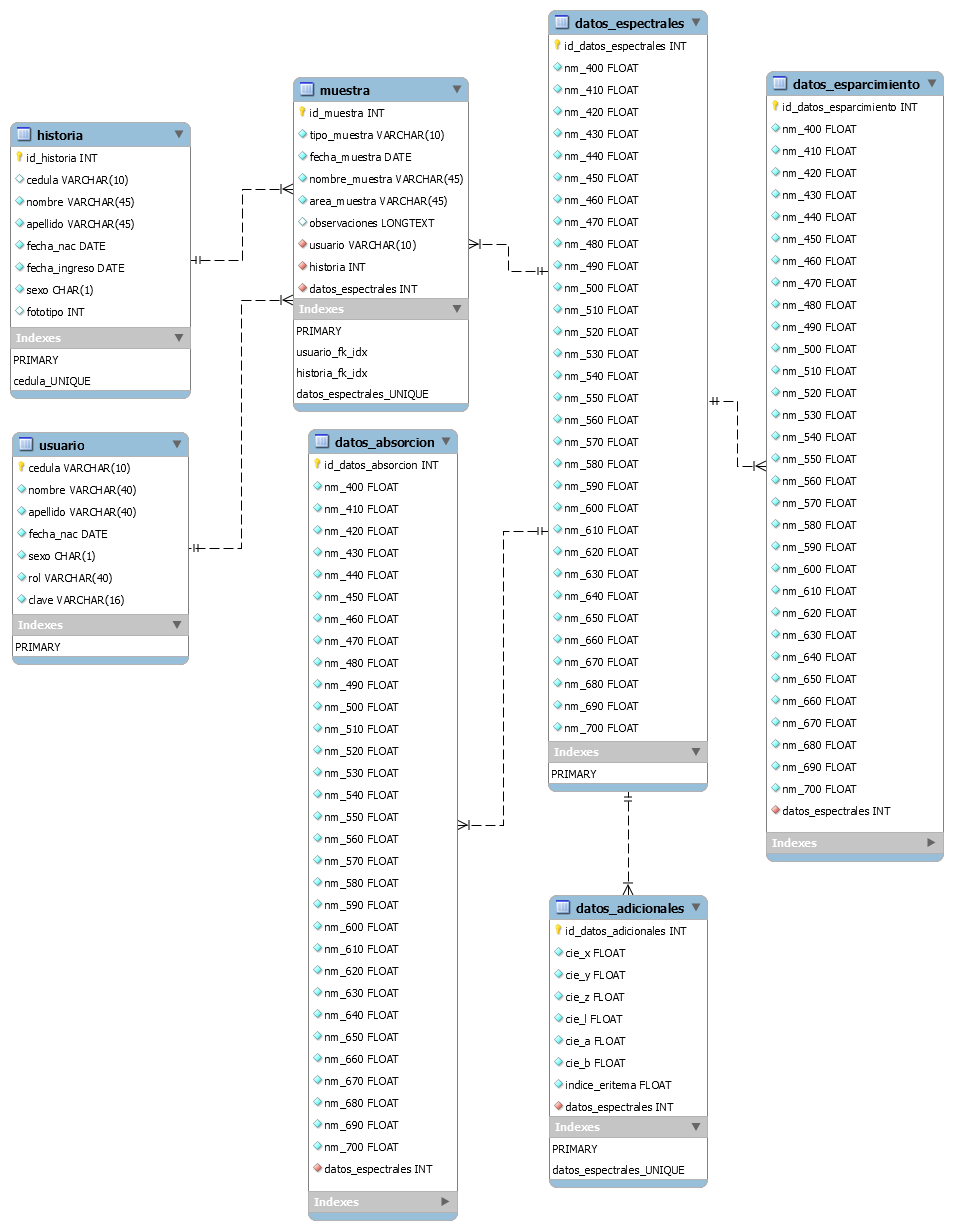
\includegraphics[scale=0.4]{img/diagramaER.png}
			\caption[Diagrama ER de la base de datos]{\textit{Diagrama ER de la base de datos} (Fuente: Autor).}
	\end{figure}
	
	\subsection{Descripci\'{o}n de las tablas de la base de datos}
	
		\begin{itemize}
				
				\item \textbf{historia:} almacena los datos referentes a la historia m\'{e}dica de cada uno de los pacientes registrados.
				
				\item \textbf{usuario:} guarda la informaci\'{o}n de cada uno de los usuarios que pueden acceder al software, que pueden ser administradores, dermat\'{o}logos o investigadores.
				
				\item \textbf{muestra:} contiene los datos relevantes de las muestras que son tomadas a los pacientes. Dichas muestras siempre est\'{a}n interrelacionadas con la historia m\'{e}dica del paciente al que pertenece, y la c\'{e}dula del usuario que la tom\'{o}.

				\item \textbf{datos\_espectrales:} contiene los 31 puntos espectrales resultantes de la medici\'{o}n realizada de cada muestra por medio del MiniScan XE Plus.
				
				\item \textbf{datos\_absorcion:} contiene los 31 puntos espectrales resultantes del c\'{a}lculo del coeficiente de absorci\'{o}n asociado con los datos espectrales.
				
				\item \textbf{datos\_esparcimiento:} contiene los 31 puntos espectrales resultantes del c\'{a}lculo del coeficiente de esparcimiento asociado con los datos espectrales.
				
				\item \textbf{datos\_adicionales:} almacena los datos que son calculados a partir de los 31 puntos espectrales de cada muestra, estos son las coordenadas de cromaticiad CIE xyz, las coordenadas del espacio del color CIELAB y el \'{i}ndice de eritema.
				
		\end{itemize}

\section{Tecnolog\'{i}as y recursos utilizados}

	\subsection{Tecnolog\'{i}as}
	
		\begin{itemize}
			
			\item \textbf{Qt:} es un \textit{framework} de desarrollo de aplicaciones multiplataforma para sistemas operativos de escritorio, sistemas integrados y sistemas m\'{o}viles. Se utiliz\'{o} la versi\'{o}n \textit{open source} 5.4.1 de este \textit{framework} para el desarrollo del Spectrasoft.
			
			\item \textbf{Visual Studio:} es un entorno integrado de desarrollo o \textit{IDE} para crear aplicaciones en varias plataformas, como Windows, Android y iOS. La versi\'{o}n 2013 de este \textit{IDE} fue utilizada para desarrollar una librer\'{i}a escrita en Visual Basic.NET, la cual act\'{u}a como intermediaria entre el kit \textit{MSXE.ocx} y el \textit{framework} Qt, para as\'{i} utilizar las caracter\'{i}sticas del MiniScan XE Plus en el Spectrasoft.
			
			\item \textbf{PostgreSQL:} es un sistema \textit{open source} multiplataforma de bases de datos relacionales. Posee m\'{a}s de 15 a\~{n}os de desarrollo activo y una arquitectura comprobada que se ha ganado una fuerte reputaci\'{o}n por confiabilidad, integridad de datos y correctitud. Este sistema se utiliz\'{o} para desarrollar y administrar la base de datos con la que opera el Spectrasoft.
			
			\item \textbf{Gitlab:} es un servicio de control de versiones que ofrece alojamiento gratuito, tanto p\'{u}blico como privado, de respositorios para proyectos. Se utiliz\'{o} la versi\'{o}n en l\'{i}nea de este servicio para llevar un control de versiones durante el desarrollo del proyecto.
			
			\item \textbf{QCustomPlot:} es un \textit{widget open source} para Qt que permite realizar el trazado y la visualizaci\'{o}n de datos. Este \textit{widget} fue empleado por el Spectrasoft para visualizar la curva de reflectancia difusa y la curva de absorbancia aparente asociadas a los 31 puntos espectrales resultantes de las mediciones.
			
			\item \textbf{QtXlsx:} es una librer\'{i}a \textit{open source} para Qt que permite leer y escribir archivos con extensi\'{o}n xlsx. Esta librer\'{i}a fue utilizada para implementar en el Spectrasoft la opci\'{o}n de exportar los resultados de una muestra a un archivo port\'{a}til, manejable por medio de aplicaciones de hojas de c\'{a}lculo.
		\end{itemize}
	
	\subsection{Recursos}
	
		\begin{itemize}
		
			\item \textbf{MiniScan XE Plus:} es un instrumento de medici\'{o}n del color creado por la empresa HunterLab, de dise\~{n}o compacto y port\'{a}til, que emplea la t\'{e}cnica de espectroscop\'{i}a de reflectancia difusa, el cual se puede apreciar en la figura 4.8. Este instrumento mide la cantidad de luz que refleja una muestra dentro de un rango de longitudes de onda que va desde los 400 hasta los 700 nan\'{o}metros, generando como resultado 31 puntos espectrales dentro de ese rango, que son el insumo principal del Spectrasoft.
			
			\item \textbf{Adaptador RS232-USB:} es un cable adaptador que habilita la comunicaci\'{o}n de dispositivos que utilizan puerto serial con computadoras que disponen de puertos USB, creando puertos COM virtuales con las mismas mientras se realiza dicha comunicaci\'{o}n. Este cable es utilizado como adaptador para el cable de comunicaci\'{o}n RS232 DB-9 hembra a RJ-45 del MiniScan XE Plus, y as\'{i} habilitar la utilizaci\'{o}n de este instrumento en computadoras que no poseen puerto serial.
			
		\end{itemize}
		
	\begin{figure}[H]
		\centering
		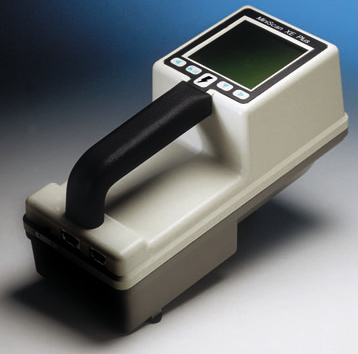
\includegraphics[scale=1]{img/MiniScanXEPlus.png}
			\caption[MiniScan XE Plus]{\textit{MiniScan XE Plus} (Fuente: HunterLab, 2006).}
	\end{figure}
	
\section{F\'{o}rmulas implementadas}
	A continuaci\'{o}n se muestra el c\'{o}digo fuente de las f\'{o}rmulas de \'{o}ptica y colorimetr\'{i}a que fueron definidas en las bases te\'{o}ricas, e implementadas en el Spectrasoft.
	
	\begin{itemize}
	
	\item \textbf{Funci\'{o}n de \'{i}ndice de eritema:}	
		\begin{lstlisting}
//Calcula el indice de eritema
float eritema(QVector<float> medicion){
    //promRojo: promedio ponderado del color rojo
    float promRojo = (medicion[24]/2.0 + medicion[25]
    + medicion[26] + medicion[27]/2.0)/3.0;

    //promVerde: promedio ponderado del color verde
    float promVerde = (medicion[16]/2.0 + medicion[17]
     + medicion[18]/2.0)/2.0;

    float resultado = 100.0*(log(1.0/promVerde)
     - log(1.0/promRojo));

    return resultado;
}
	\end{lstlisting}
	
\newpage	
	
		\item \textbf{Funci\'{o}n de absorbancia aparente:}
			\begin{lstlisting}
//Calcula los datos de absorbancia aparente
QVector<float> absorbancia(QVector<float> medicion){

	QVector<float> resultado;
	
   	for(int i = 0; i < 31; ++i)
		resultado.push_back(100.0 - medicion[i]);

    return resultado;
}
			\end{lstlisting}
			
		\item \textbf{Funci\'{o}n de coordenadas de cromaticidad CIE xyz:}		
			\begin{lstlisting}
//Calcula las coordenadas de cromaticidad CIE xyz
QVector<float> CIExyz(QVector<float> medicion){
    
    QVector<float> resultado;
    QVector<float> XYZ = CIEXYZ(medicion);
    float x, y, z;

    x = XYZ[0]/(XYZ[0] + XYZ[1] + XYZ[2]);
    y = XYZ[1]/(XYZ[0] + XYZ[1] + XYZ[2]);
    z = XYZ[2]/(XYZ[0] + XYZ[1] + XYZ[2]);

    resultado.push_back(x);
    resultado.push_back(y);
    resultado.push_back(z);

    return resultado;
}
			\end{lstlisting}
			
\newpage
		
		\item \textbf{Funci\'{o}n de valores triest\'{i}mulo CIE XYZ:}
			\begin{lstlisting}
//Calcula los valores triestimulo CIE XYZ
QVector<float> CIEXYZ(QVector<float> medicion){
    
    QVector<float> resultado;
    float auxK, auxX, auxY, auxZ, k, X, Y, Z;

    auxK = auxX = auxY = auxZ = 0.0;

    //realiza las sumatorias indicadas de las formulas
    for(int i = 0; i < 31; ++i){

		auxK+= iluCIED65[i]*yCIE10[i];
        auxX+= medicion[i]*iluCIED65[i]*xCIE10[i];
        auxY+= medicion[i]*iluCIED65[i]*yCIE10[i];
        auxY+= medicion[i]*iluCIED65[i]*zCIE10[i];
    }

    //calcula la constante k
    k = 100.0/auxK;

    //calcula los valores triestimulo XYZ
    X = k*auxX;
    Y = k*auxY;
    Z = k*auxZ;

    resultado.push_back(X);
    resultado.push_back(Y);
    resultado.push_back(Z);

    return resultado;
}
			\end{lstlisting}

\newpage
		
		\item \textbf{Funci\'{o}n de coordenadas CIELAB:}
			\begin{lstlisting}
//Calcula las coordenadas de del espacio CIELAB
QVector<float> CIELAB(QVector<float> medicion){
    
    QVector<float> resultado;
    QVector<float> XYZ = CIEXYZ(medicion);
    float constante, aux, fXfYfZ[3], L, a, b;

    //calcula la constante utilizada en la formula
    constante = 24.0/116.0;
    constante = pow(constante, 3);

    //calcula las funciones X/Xn, Y/Yn, Z/Zn
    for(int i = 0; i < 3; ++i){

        aux = XYZ[i]/XnYnZn[i];

        if(aux > constante){
            fXfYfZ[i] = pow(aux, 1.0/3.0);
        }else{
            fXfYfZ[i] = (841.0/108.0)*aux + (16.0/116.0);
        }
    }

    //calcula las coordenadas L*a*b*
    L = 116.0*fXfYfZ[1] - 16.0;
    a = 500.0*(fXfYfZ[0] - fXfYfZ[1]);
    b = 200.0*(fXfYfZ[1] - fXfYfZ[2]);

    resultado.push_back(L);
    resultado.push_back(a);
    resultado.push_back(b);

    return resultado;
}
		\end{lstlisting}

	\end{itemize}

\newpage

\section{Interfaz del Spectrasoft}

	A continuaci\'{o}n se muestran algunas de las vistas de la interfaz gr\'{a}fica de usuario del Spectrasoft, que comprenden la vista principal, la ventana de inicio de sesi\'{o}n de un usuario, la visualizaci\'{o}n de algunos de los resultados de una medici\'{o}n realizada, y los detalles de la historia m\'{e}dica de un paciente.

 \begin{itemize}
 	
 	\item \textbf{Vista principal:}
 	
 		\begin{figure}[H]
		\centering
		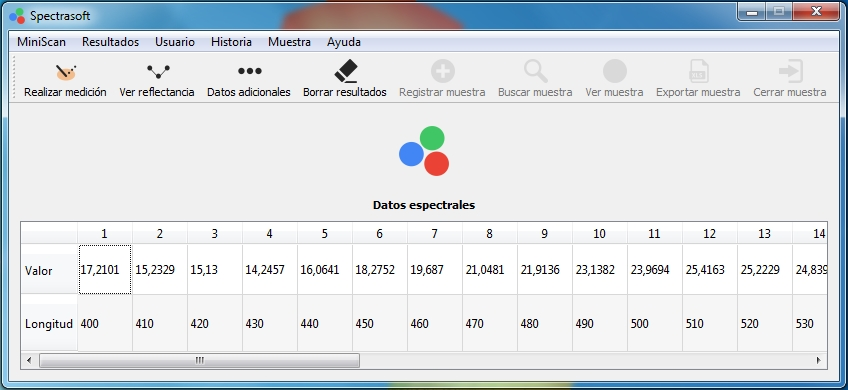
\includegraphics[scale=0.6]{img/vista-principal.jpg}
			\caption[Vista principal del Spectrasoft]{\textit{Vista principal del Spectrasoft} (Fuente: Autor).}
	\end{figure}
	
	 	\item \textbf{Inicio de sesi\'{o}n:}
 	
 		\begin{figure}[H]
		\centering
		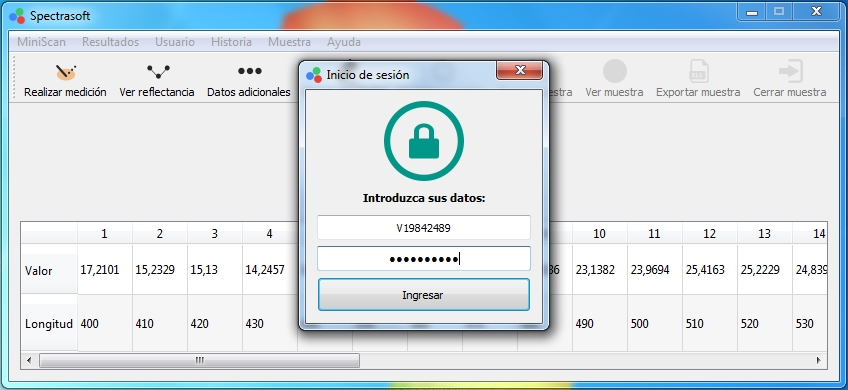
\includegraphics[scale=0.6]{img/vista-inicio-sesion.jpg}
			\caption[Inicio de sesi\'{o}n del Spectrasoft]{\textit{Inicio de sesi\'{o}n del Spectrasoft} (Fuente: Autor).}
	\end{figure}

\newpage
	 	\item \textbf{Curva de reflectancia y datos adicionales:}
 	
 		\begin{figure}[H]
		\centering
		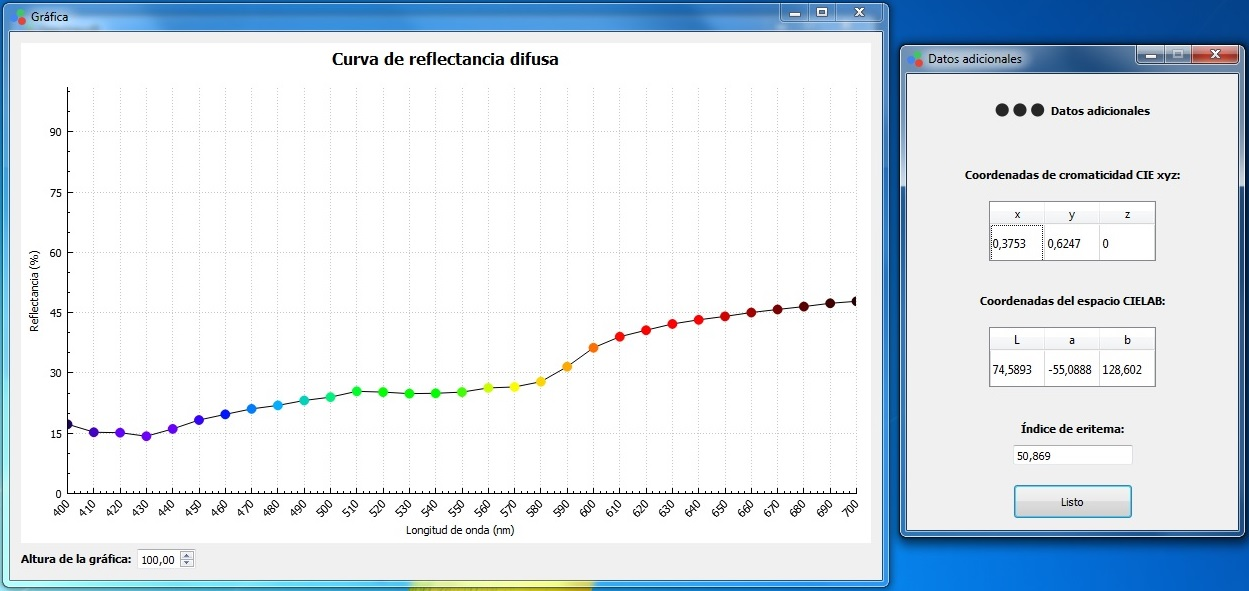
\includegraphics[scale=0.4]{img/vista-resultados.jpg}
			\caption[Curva de reflectancia y datos adicionales]{\textit{Curva de reflectancia y datos adicionales} (Fuente: Autor).}
	\end{figure}
	
		 	\item \textbf{Historia m\'{e}dica de un paciente:}
 	
 		\begin{figure}[H]
		\centering
		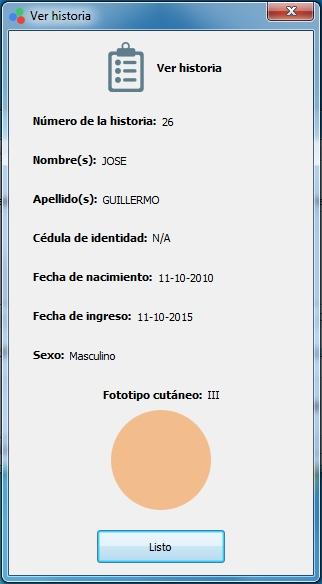
\includegraphics[scale=0.6]{img/vista-historia.jpg}
			\caption[Historia m\'{e}dica de un paciente]{\textit{Historia m\'{e}dica de un paciente} (Fuente: Autor).}
	\end{figure}

\end{itemize}

\newpage

\section{Pruebas realizadas}

	\newpage
	\chapter{Conclusiones y recomendaciones}

\section{Conclusiones}

	La elaboraci\'{o}n de la presente investigaci\'{o}n ha cumplido los objetivos planteados. Para lograr esto fue necesario un an\'{a}lisis detallado de la bibliograf\'{i}a, la revisi\'{o}n de algunas investigaciones previas, y el estudio riguroso del material proporcionado por el personal de soporte t\'{e}cnico de la empresa HunterLab.
	
	El aporte general de este trabajo de investigaci\'{o}n se centra en proveer un software libre para operar el MiniScan XE Plus, el cual dispone de las funciones necesarias para que los dermat\'{o}logos puedan establecer diagn\'{o}sticos de patolog\'{i}as dermatol\'{o}gicas en pacientes.
	
	Desde el comienzo del proceso de desarrollo del software se opt\'{o} por trabajar con un servicio gratuito de control de versiones, lo cual permiti\'{o} tener almacenado el c\'{o}digo fuente del software de manera centralizada. Esto ayud\'{o} a tener una mejor organizaci\'{o}n durante el desarrollo.
	
	Debido a las limitaciones encontradas durante la investigaci\'{o}n, se concluye que es necesaria la utilizaci\'{o}n de algunos archivos de HunterLab para lograr la comunicaci\'{o}n entre el software resultante y el MiniSan XE Plus. Adicionalmente, debido a esta limitaci\'{o}n el software resultante no puede captar ni interpretar las se\~{n}ales de los botones del MiniScan XE Plus, ya que estos archivos no ofrecen esta caracter\'{i}stica para ser utilizada fuera del HunterLab Universal Software.
	
	La instalaci\'{o}n de este software no es tan simple como podr\'{i}a llegar a ser, como consecuencia de la necesidad de utilizar algunos archivos del HunterLab. El software resultante no puede habilitarse para ser multiplataforma debido a esta raz\'{o}n.

	Durante las pruebas de funcionalidad y usabilidad realizadas al software se hizo notorio el nivel de aceptaci\'{o}n y la satisfacci\'{o}n de los clientes a los que iba dirigido. Adicionalmente, se realiz\'{o} un manual de usuario para la correcta utilizaci\'{o}n del software, que explica detalladamente con tablas y con im\'{a}genes la permisolog\'{i}a de sus usuarios y las funciones que ofrece, por lo que su curva de aprendizaje es baja.

	En definitiva, se concluye que el software resultante cumple con todos los objetivos establecidos en esta investigaci\'{o}n, ajustandose a las necesidades de los dermat\'{o}logos, garantizando un mejor aprovechamiento del MiniScan XE Plus, creando una base sobre la cual se pueden realizar trabajos futuros que modifiquen, mejoren y extiendan dicho software.

\newpage

\section{Recomendaciones}

	De acuerdo a las conclusiones alcanzadas con el trabajo, se han generado una serie de recomendaciones, las cuales se presentan a continuaci\'{o}n.

\begin{itemize}

	\item Permitir la visualizaci\'{o}n, consulta y exportaci\'{o}n de varias muestras al mismo tiempo.
	
	\item Desarrollar un arhivo controlador para el MiniScan XE Plus que no dependa del kit MSXE.ocx del HunterLab, para as\'{i} simplificar el proceso de instalaci\'{o}n del Spectrasoft, lograr que el mismo sea capaz de captar e interpretar las se\~{n}ales de los botones del MiniScan XE Plus, y posibilitar que \'{e}ste sea multiplataforma.
	
	\item Incluir la f\'{o}rmula desarrollada por los investigadores del CIMBUC para el c\'{a}lculo del coeficiente de esparcimiento de la epidermis, la cual no estuvo lista durante el tiempo en el que se llev\'{o} a cabo este trabajo de investigaci\'{o}n.
	
	\item Crear una nueva base de datos que habilite la gesti\'{o}n de muestras experimentales para los investigadores del CIMBUC.
	
	\item Adaptar el Spectrasoft a una arquitectura de modelo cliente-servidor para permitir la conexi\'{o}n con bases de datos remotas en sistemas distribuidos.
	
	\item Disponer de un ambiente \textit{QA} para realizar pruebas de rendimiento y de base de datos al Spectrasoft, previas a su puesta en producci\'{o}n.
	
	\item Incluir la carga de muestras por archivo al Spectrasoft.
\end{itemize}
	\newpage
	\nocite{*}
	\renewcommand\bibname{Referencias}
	\bibliography{bibliografia}
\end{document}